\documentclass{report}

%pacchetti
\usepackage[utf8]{inputenc}
\usepackage[italian]{babel}
%permette ai riferimenti di essere cliccabili
\usepackage{hyperref}
%permette di fare riferimento a un elemento tramite il suo nome
\usepackage{nameref}
%impostazione dei margini del documento
\usepackage[margin=1in]{geometry}
%inserimento di immagini
\usepackage{graphics}

%inserimento di pezzi di codice
\usepackage{listings}
%colori per il codice
\usepackage{xcolor}

%impostazioni dei collegamenti ipertestuali
\hypersetup{
    colorlinks=true,
    linkcolor=blue,
    filecolor=blue,
}

\urlstyle{same}

%impostazione della profondità a cui mostrare le parti del documento nell'indice
\setcounter{tocdepth}{3}
\setcounter{secnumdepth}{3}

%setup colori e visualizzazione codice
\definecolor{codegray}{rgb}{0.5,0.5,0.5}
\definecolor{lgray}{rgb}{0.95,0.95,0.95}

\lstdefinestyle{mystyle}{
    backgroundcolor=\color{lgray},   
    commentstyle=\color{cyan},
    keywordstyle=\color{blue},
    numberstyle=\color{codegray},
    stringstyle=\color{orange},
    breakatwhitespace=false,         
    breaklines=true,                                   
    keepspaces=true,                 
    numbers=left,                    
    numbersep=5pt,                  
    showspaces=false,                
    showstringspaces=false,
    showtabs=false,                  
    tabsize=2
}

\lstset{style=mystyle}

%disabilitazione dell'indentazione a inizio paragrafo
\setlength{\parindent}{0pt}

\title{Meteo in Tempo Reale}
\author{Matteo Celardo 984457}
\date{PWM - secondo semestre A.A. 2021/2022}

\begin{document}

\maketitle

% Indice
\tableofcontents

\chapter{Introduzione}

\section{Analisi dei requisiti}

\subsection{Destinatari}

L'applicazione è progettata per andare incontro a qualunque tipo di utente, dal più al meno esperto, grazie ad 
un'interfaccia semplice ed intuitiva, la quale permette di trovare facilmente le informazioni relative al meteo in tempo reale 
della città a cui si è interessati tramite la barra di ricerca o tramite le città impostate tra i propri preferiti, previa 
registrazione e introduzione delle stesse nell'apposito spazio all'interno dell'area personale.

\vspace{5mm}

Nella versione attuale, non sono posti particolari vincoli di banda grazie alla sola presenza degli elementi utili alla 
navigazione, riducendo così la latenza il più possibile. Inoltre, le immagini relative alle condizioni metereologiche delle città 
visualizzate saranno caricate in modalità asincrona, riducendo al minimo il periodo in cui la pagina non risponde agli input 
dell'utente.\\
Attualmente, si consiglia la navigazione via PC per una maggiore semplicità di lettura, ma è comunque possibile utilizzare un 
telefono grazie alla responsività degli elementi presenti nelle pagine.

\vspace{5mm}

Gli utenti che si recano sulla piattaforma web saranno principalmente persone che hanno la necessità di sapere le condizioni 
meteo di una città di loro interesse, motivo per cui i contenuti sono organizzati in modo tale da fornire informazioni su 
richiesta esplicita dell'utente tramite una barra di ricerca oppure tramite gli elementi salvati nell'area personali una volta 
effettuato il login


\subsection{Modello di valore}

L'applicazione si contraddistingue per essere intuitiva e veloce da usare, elementi sempre graditi durante l'esperienza utente.

\vspace{5mm}

Grazie alla disponibilità in tempo reale di informazioni relative al tempo, quest'applicazione potrebbe essere integrata con 
un'API in grado di fornire informazio a sistemi automatici in grado usati per svolgere operazioni in base al tempo atmosferico, 
risparmiando così ingenti somme di denaro in sensori e cablaggi.\\
Benché attualmente non presenti, sarebbe facile inserire banner pubblicitari o sponsor di sorta grazie alla struttura modulare 
del progetto.\\
Entrambi questi elementi accrescerebbero notevolmente il valore economico dell'applicazione in dipendenza, rispettivamente, al 
numero di sistemi automatici collegabili per utente o al numero di banner inseriti, motivo per cui risulta difficile formulare 
una stima esatta di valore economico.

\subsection{flusso di dati}

Il flusso dei dati all'interno dell'applicazione é unicamente in formato JSON: lo scambio di dati tra client e server o tra 
client e API di siti esterni é infatti interamente gestito attraverso l'inoltro di oggetti e stringhe JSON.\\
Grazie ad una struttura REST, le comunicazioni saranno unicamente aperte dal client nel momento in cui necessiterà di una risorsa 
(come il meteo relativo ad una città oppure un'altra pagina del sito), il quale richiederà ciò di cui necessita tramite 
oggetti JSON inviati al server, ricevendone altri in risposta che permetteranno di agiornare un frammento della pagina o di effettuare 
il reindirizzamento.

\vspace{5mm}

I contenuti salvati sono interamente archiviati lato server tramite l'uso di un database MongoDB ad eccezione della preferenza 
espressa dall'utente per vare la pagina in dark mode oppure in light mode, i quali sono salvati localmente attraverso 
localStorage.

\vspace{5mm}

Allo stato attuale, il progetto prevede solo costi per la manutenzione in up del server, senza che siano necessari particolari 
interventi di manutenzione periodici. 

\vspace{5mm}

Il progetto utilizza unicamente librerie e API reperibili gratuitamente, ma sarebbe perfettamente possibile modificarle ed 
adottarne di colsed source a pagamento con pochi e semplici aggiustamenti grazie ad una gestione modulare del codice.


\subsection{Aspetti tecnologici}

La trasmissione di dati può essere effettuata in chiaro ad eccezione della password usata per accedere alla propria area 
personale, la quale viene trasmessa sotto forma di SHA256 per evitare che sia leggibile.

\vspace{5mm}

Il database prevede la creazione di una singola collezione contenente:
\begin{itemize}
    \item \emph{\_id}: id univoco assegnato dal database in automatico;
    \item \emph{user}: username;
    \item \emph{email}: email dell'utente;
    \item \emph{pw}: password dell'utente sotto forma di digest SHA256;
    \item \emph{pref}: array contenente le città messe tra i preferiti dall'utente. può essere vuoto.
\end{itemize}

\vspace{5mm}

Tecnologie utilizzate:
\begin{itemize}
    \item \emph{HTML 5 e bootstrap}: realizzazione della struttura delle pagine e gestione degli stili con bootstrap;
    \item \emph{JavaScript}: realizzazione delle richiese al server e alle API, nonché del toggle della darkmode e l'aggiornamento 
    di frammenti di pagina con dati ricevuti dal server; 
    \item \emph{Node JS}: implementazione del server con tutte le sue funzionalità (caricamento di tutte le pagine, 
    invio di oggetti JSON per aggiornare frammenti di pagina, interrogazione dell'API per ottenere il nome dei comuni e delle 
    regioni italiani);
    \item \emph{Express}: framework utilizzato per semplificare il deploy del serever;
    \item \emph{JSON}: formato usato per la trasmissione dei dati;
    \item \emph{localStorage}: usato per il salvataggio della preferenza utente per la visualizzazione della pagina (dark o light mode)
    \item \emph{MongoDB}: database utilizzato per salvare le informazioni relative agli utenti registrati sull'app;
    \item \emph{API}: nel progetto sono state utilizzate 2 API:
    \begin{itemize}
        \item \emph{pexels}: API utilizzata per reperire le immagini mostrate nelle pagine;
        \item \emph{comuni ITA}: API usata per ottenere i nomi di regioni, province e comuni italiani.
    \end{itemize}
\end{itemize}


\chapter{Interfacce}

Per realizzare le pagine sono stati usati \emph{HTML 5} e \emph{bootstrap}.\\ 
Gli elementi di personalizzazione, come il nome utente nella navbar una volta autenticati o il meteo 
in tempo reale delle città salvate tra i preferiti, sono inseriti utilizzando \emph{EJS}.

\vspace{5mm}

In ogni pagina, il contenuto del tag \emph{head} e alcuni script (necessari per dark mode toggle, bootstrap e 
ricerca di una città) sono aggiunti tramite l'utilizzo di \emph{partials}, elementi supportati da EJS.

\section{Index.ejs}

\begin{figure}[ht]
    \centering
    \resizebox{\textwidth}{!}{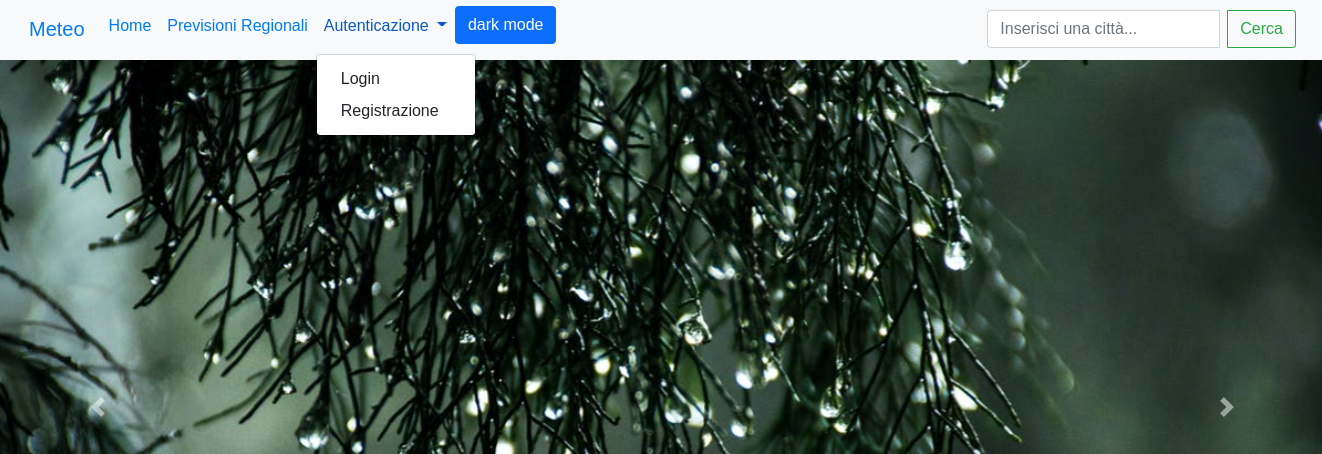
\includegraphics{img/indexSopra.png}}
    \caption{Metà superiore dell'home page}
\end{figure}

Nella metà superiore dell'index troviamo una navbar semplice ed intuitiva: abbiamo infatti la 
possibilità di vedere le previsioni delle province di ogni regione cliccando su 
\emph{Previsioni Regionali}, di autenticarci facendo il login o la registrazione tramite il menù a 
tendina apribile cliccando su \emph{Autenticazione} (menù che sarà sostituito con un altro  
a seguito del login per poter effettuare il logut e accedere all'area personale), di cambiare la visualizzazione 
della pagina dalla modalità \emph{dark mode} a quella \emph{light mode} ed infine di cercare una città tramite 
l'apposita barra di ricerca in alto a destra.\\ 
Al di sotto della navbar, troviamo uno slider temporizzato che mostra immagini relative a condizioni 
climatiche differenti. 

\newpage
\begin{figure}[ht]
    \centering
    \resizebox{\textwidth}{!}{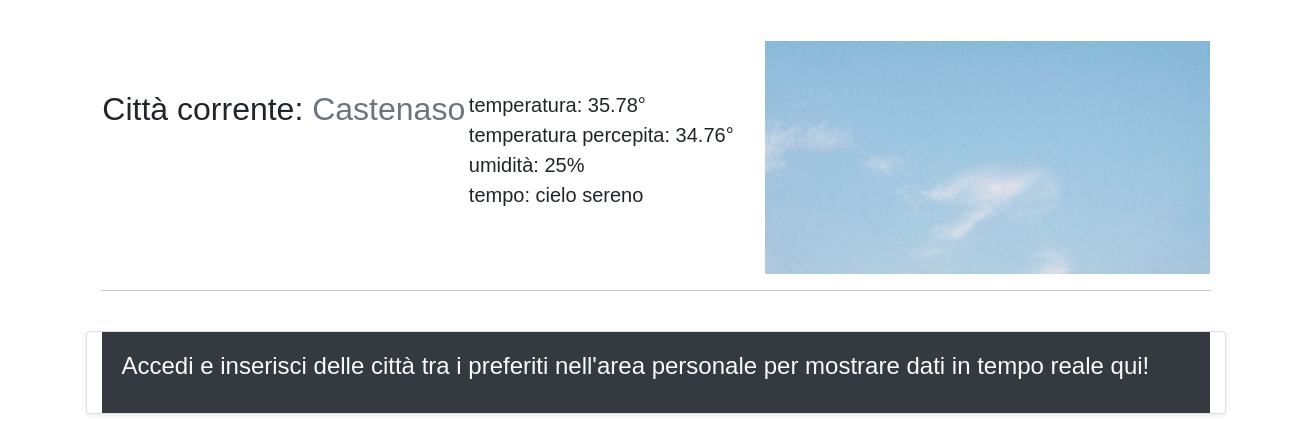
\includegraphics{img/indexSotto.png}}
    \caption{Metà inferiore dell'home page}
\end{figure}

Superato lo slider, troviamo una sezione dedicata alle condizioni meteo della città in cui ci troviamo 
(le coordinate sono ottenute con l'oggetto \emph{navigator.geolocation}, motivo per cui utilizzare una 
connessione da telefono cellulare garantirà una maggiore precisione) a seguito della quale è presente 
un'area dedicata alla visualizzazione delle città salvate tra i preferiti nell'area personale accessibile 
dopo il login.

\begin{figure}[ht]
    \centering
    \resizebox{\textwidth}{!}{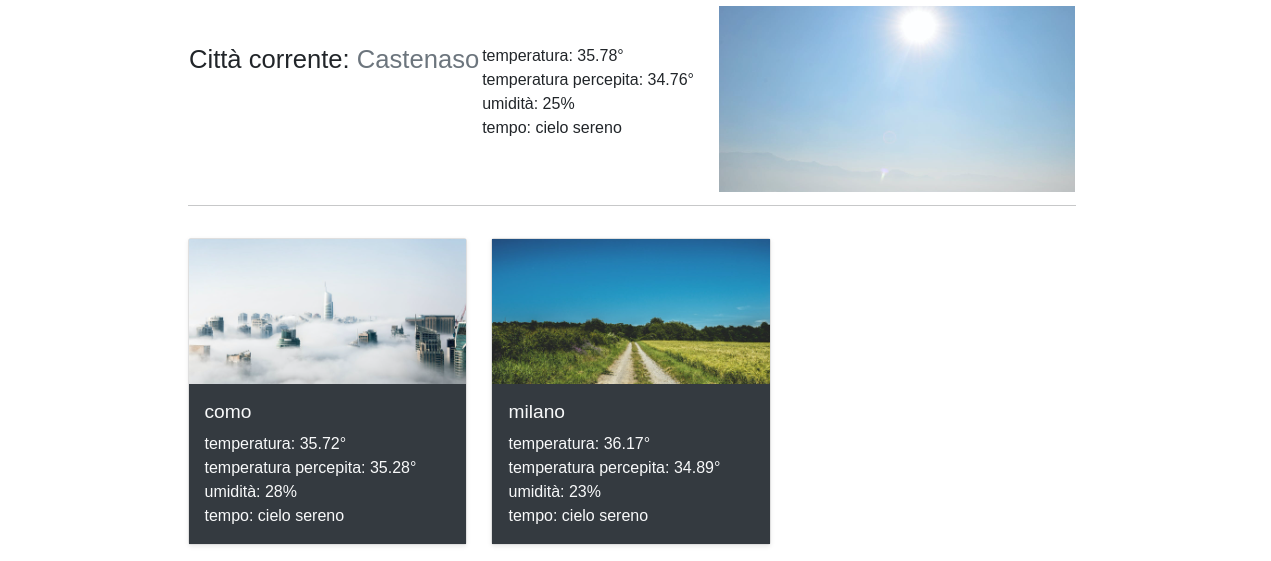
\includegraphics{img/indexLogged.png}}
    \caption{Metà inferiore dell'home page dopo aver effettuato il login}
\end{figure}

\newpage
\section{Previsioni}

\subsection{Regionali.ejs}

\begin{figure}[ht]
    \centering
    \resizebox{\textwidth}{!}{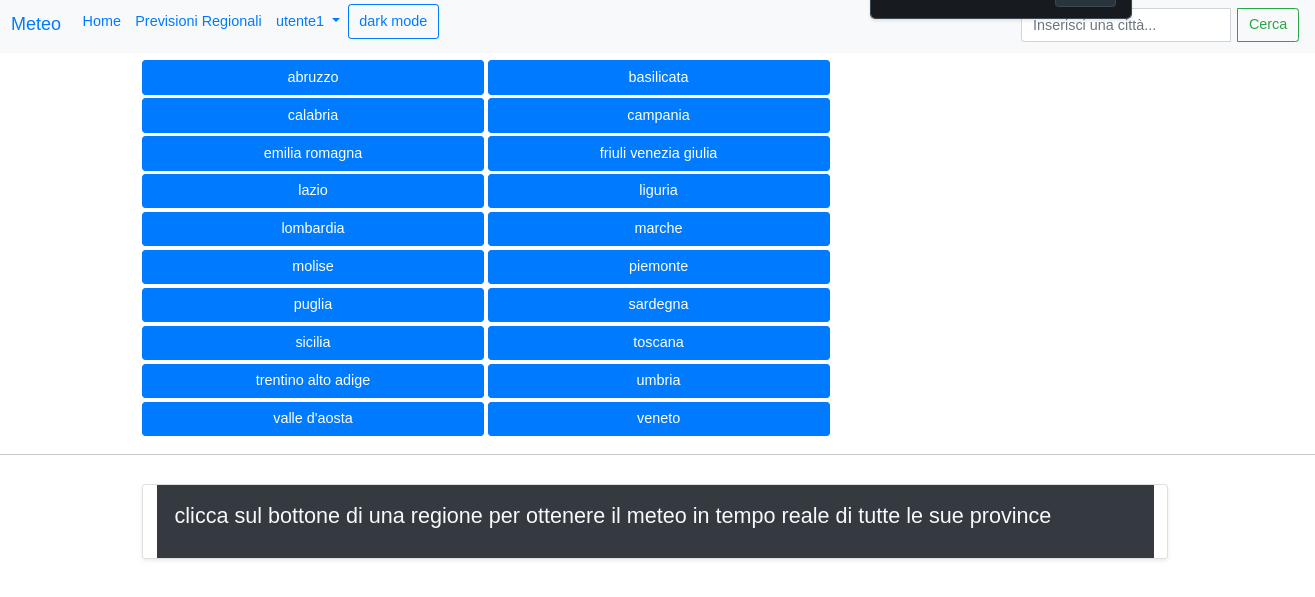
\includegraphics{img/previsioniRegionali.png}}
    \caption{Pagina dedicata alle previsioni regionali prima di cliccare su una regione}
\end{figure}

In questa pagina è possibile visualizzare le previsioni relative a tutte le province di una regione 
premendo sul tasto della regione voluta.\\
Fatto ciò, verrà visualizzato per ogni provincia un riquadro analogo a quelli presenti nell'index dopo 
il login con le informazioni metereologiche in tempo reale.

\begin{figure}[ht]
    \centering
    \resizebox{\textwidth}{!}{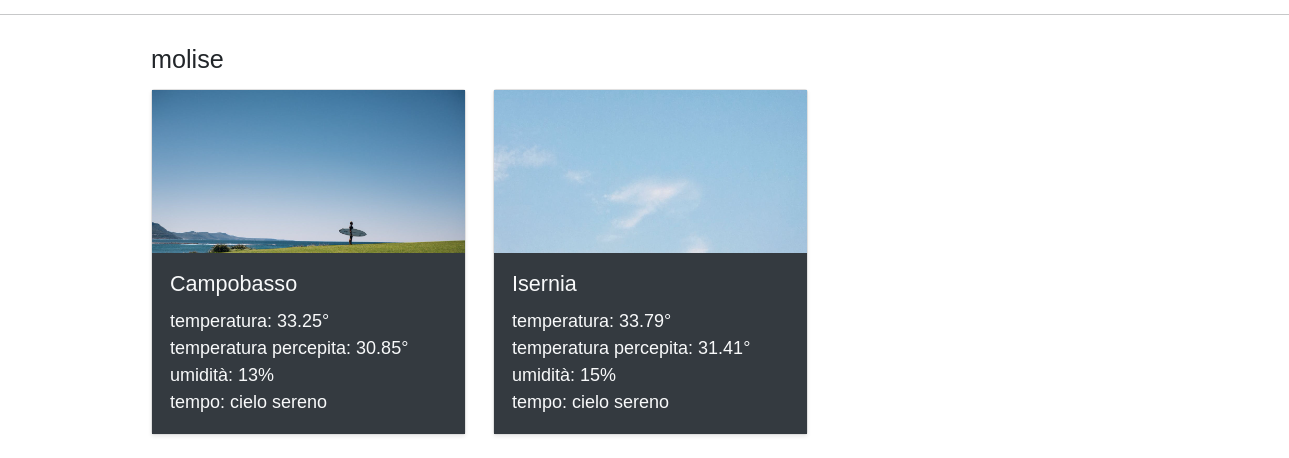
\includegraphics{img/previsioniRegionaliMolise.png}}
    \caption{Nell'immagine di esempio, la regione selezionata è stata il Molise}
\end{figure}

\newpage
\subsection{CitCercata.ejs}

\begin{figure}[ht]
    \centering
    \resizebox{\textwidth}{!}{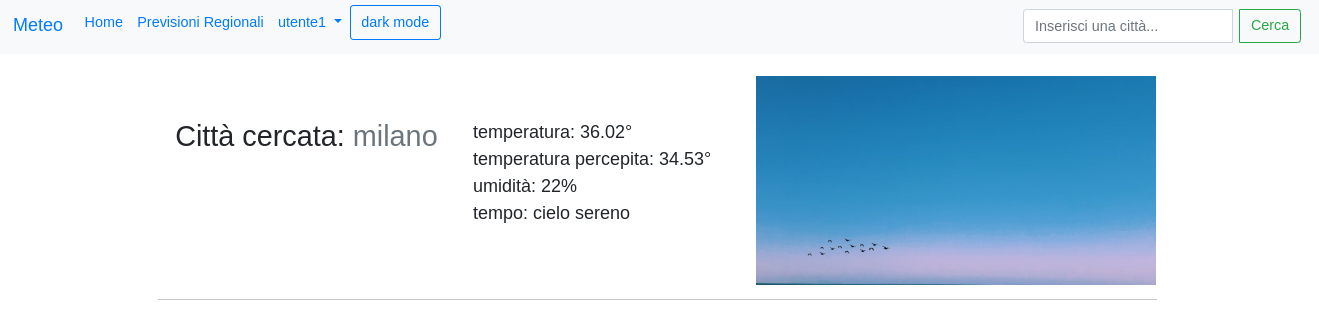
\includegraphics{img/citCercata.png}}
    \caption{Pagina visualizzata a seguito della ricerca di una città nella navbar}
\end{figure}

Attraverso la barra di ricerca in alto a destra nella navbar, è possibile cercare il nome della città per cui si 
vogliono ottenre le condzioni meteo in tempo reale.\\

\vspace{5mm}

Scrivendo il nome, verrà visualizzato a sinistra dell'input una scritta che informerà l'utente se la città inserita 
risulta esistente o meno (il sistema è strutturato per non essere \emph{case sensitive}). Nel caso in cui la città risulti 
esistente, verrà visualizzata la pagina in immagine, in caso contrario si rimarrà sulla pagina da cui si aveva fatto la ricerca.

\section{Login e Registrazione}

\subsection{Login.ejs}

\begin{figure}[ht]
    \centering
    \resizebox{\textwidth}{!}{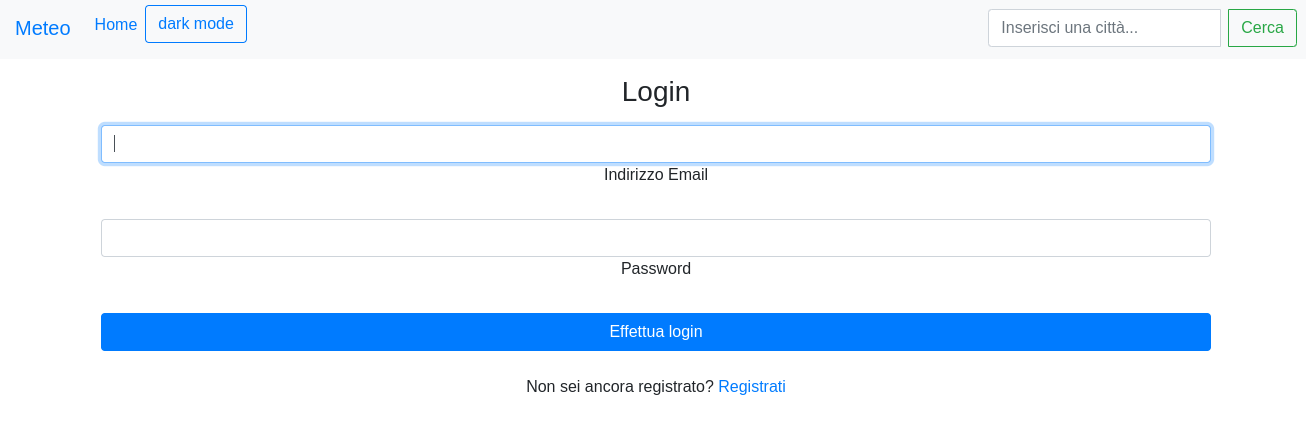
\includegraphics{img/login.png}}
    \caption{Pagina dedicata al login}
\end{figure}

Grazie a questa pagina è possibile effettuare il login nel caso si sia già registrati oppure di registrarsi attravero l'apposito 
link al di sotto del form con le credenziali.\\
La navbar è semplificata in modo da rendere l'interfaccia meno dispersiva e permette unicamente di tornare alla home, gestire 
la modalità di visualizzazione della pagina oppure cercare una città.

\newpage
\subsection{Registrazione.ejs}

\begin{figure}[ht]
    \centering
    \resizebox{\textwidth}{!}{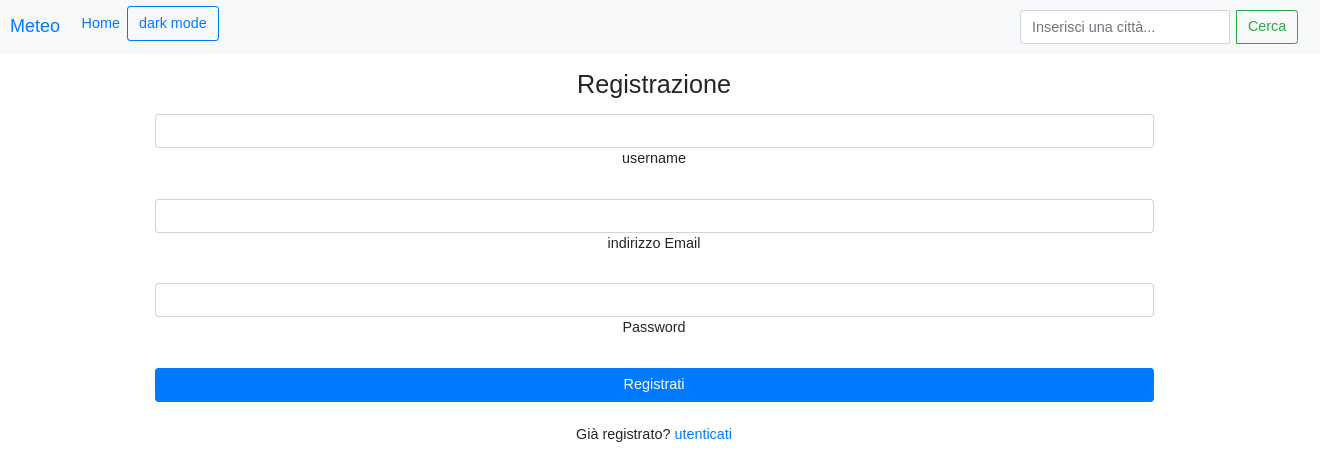
\includegraphics{img/registrazione.png}}
    \caption{Pagina dedicata alla registrazione}
\end{figure}

In questa pagina verranno richieste le credenziali usate in seguito per effettuare il login (email e password) e un nome utente. 
Questi dati saranno modificabili in un secondo momento tramite l'area personale (\textbf{N.B.}: non è possibile avere più utenti con 
la stessa mail e/o lo stesso username).\\

\vspace{5mm}

Se necessario, è possibile passare alla pagina di login tramite il link in basso.\\

\vspace{5mm}

La navbar è semplificata nella stessa maniera della pagina di login.

\subsection{AreaPersonale.ejs}

\begin{figure}[ht]
    \centering
    \resizebox{\textwidth}{!}{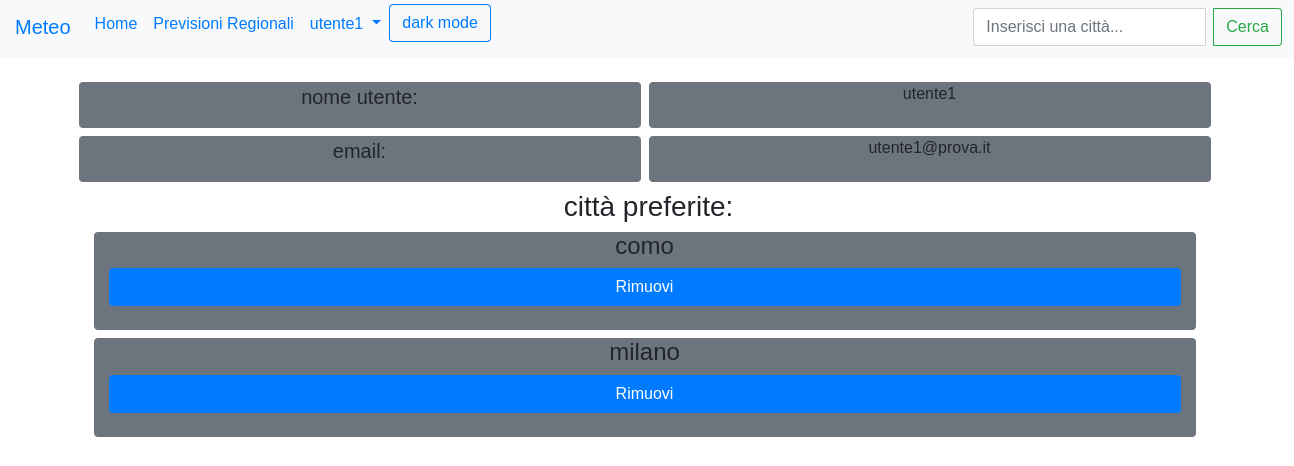
\includegraphics{img/areaPSopra.png}}
    \caption{Metà superiore della pagina dedicata all'area personale}
\end{figure}

Nella metà superiore della pagina troviamo una navbar analoga a quella presente nell'index a seguito del login.

\vspace{5mm}

Al di sotto di essa, abbiamo i dati relativi all'utente (username e email. la password non viene mostrata per ragioni di 
sicurezza) e l'elenco delle città salvate tra i preferiti, se presenti.

\begin{figure}[ht]
    \centering
    \resizebox{\textwidth}{!}{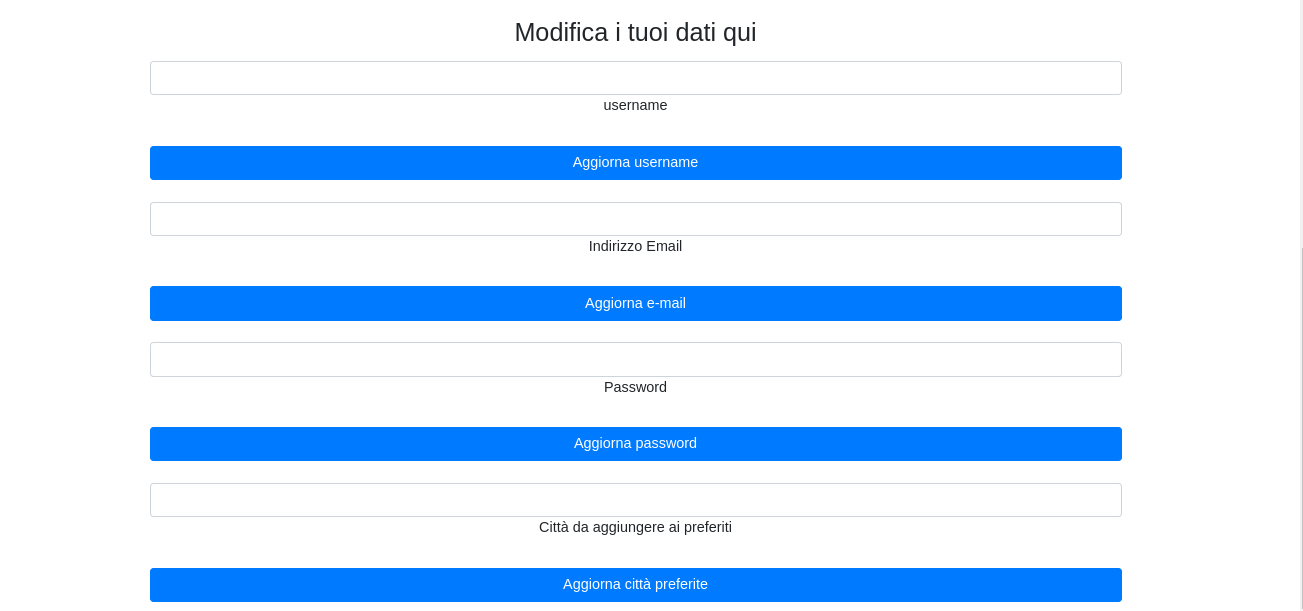
\includegraphics{img/areaPSotto.png}}
    \caption{Metà inferiore della pagina dedicata all'area personale}
\end{figure}

A seguito di queste informazioni, troviamo una serie di form che permettono, attraverso chiamate asincrone al server, di modificare 
i dati relativi all'utente, quali:
\begin{itemize}
    \item username
    \item email
    \item password 
    \item città salvate tra i preferiti
\end{itemize}
\chapter{Architettura}

\section{Struttura del sito}

\begin{figure}[ht]
    \centering
    \resizebox{\textwidth}{!}{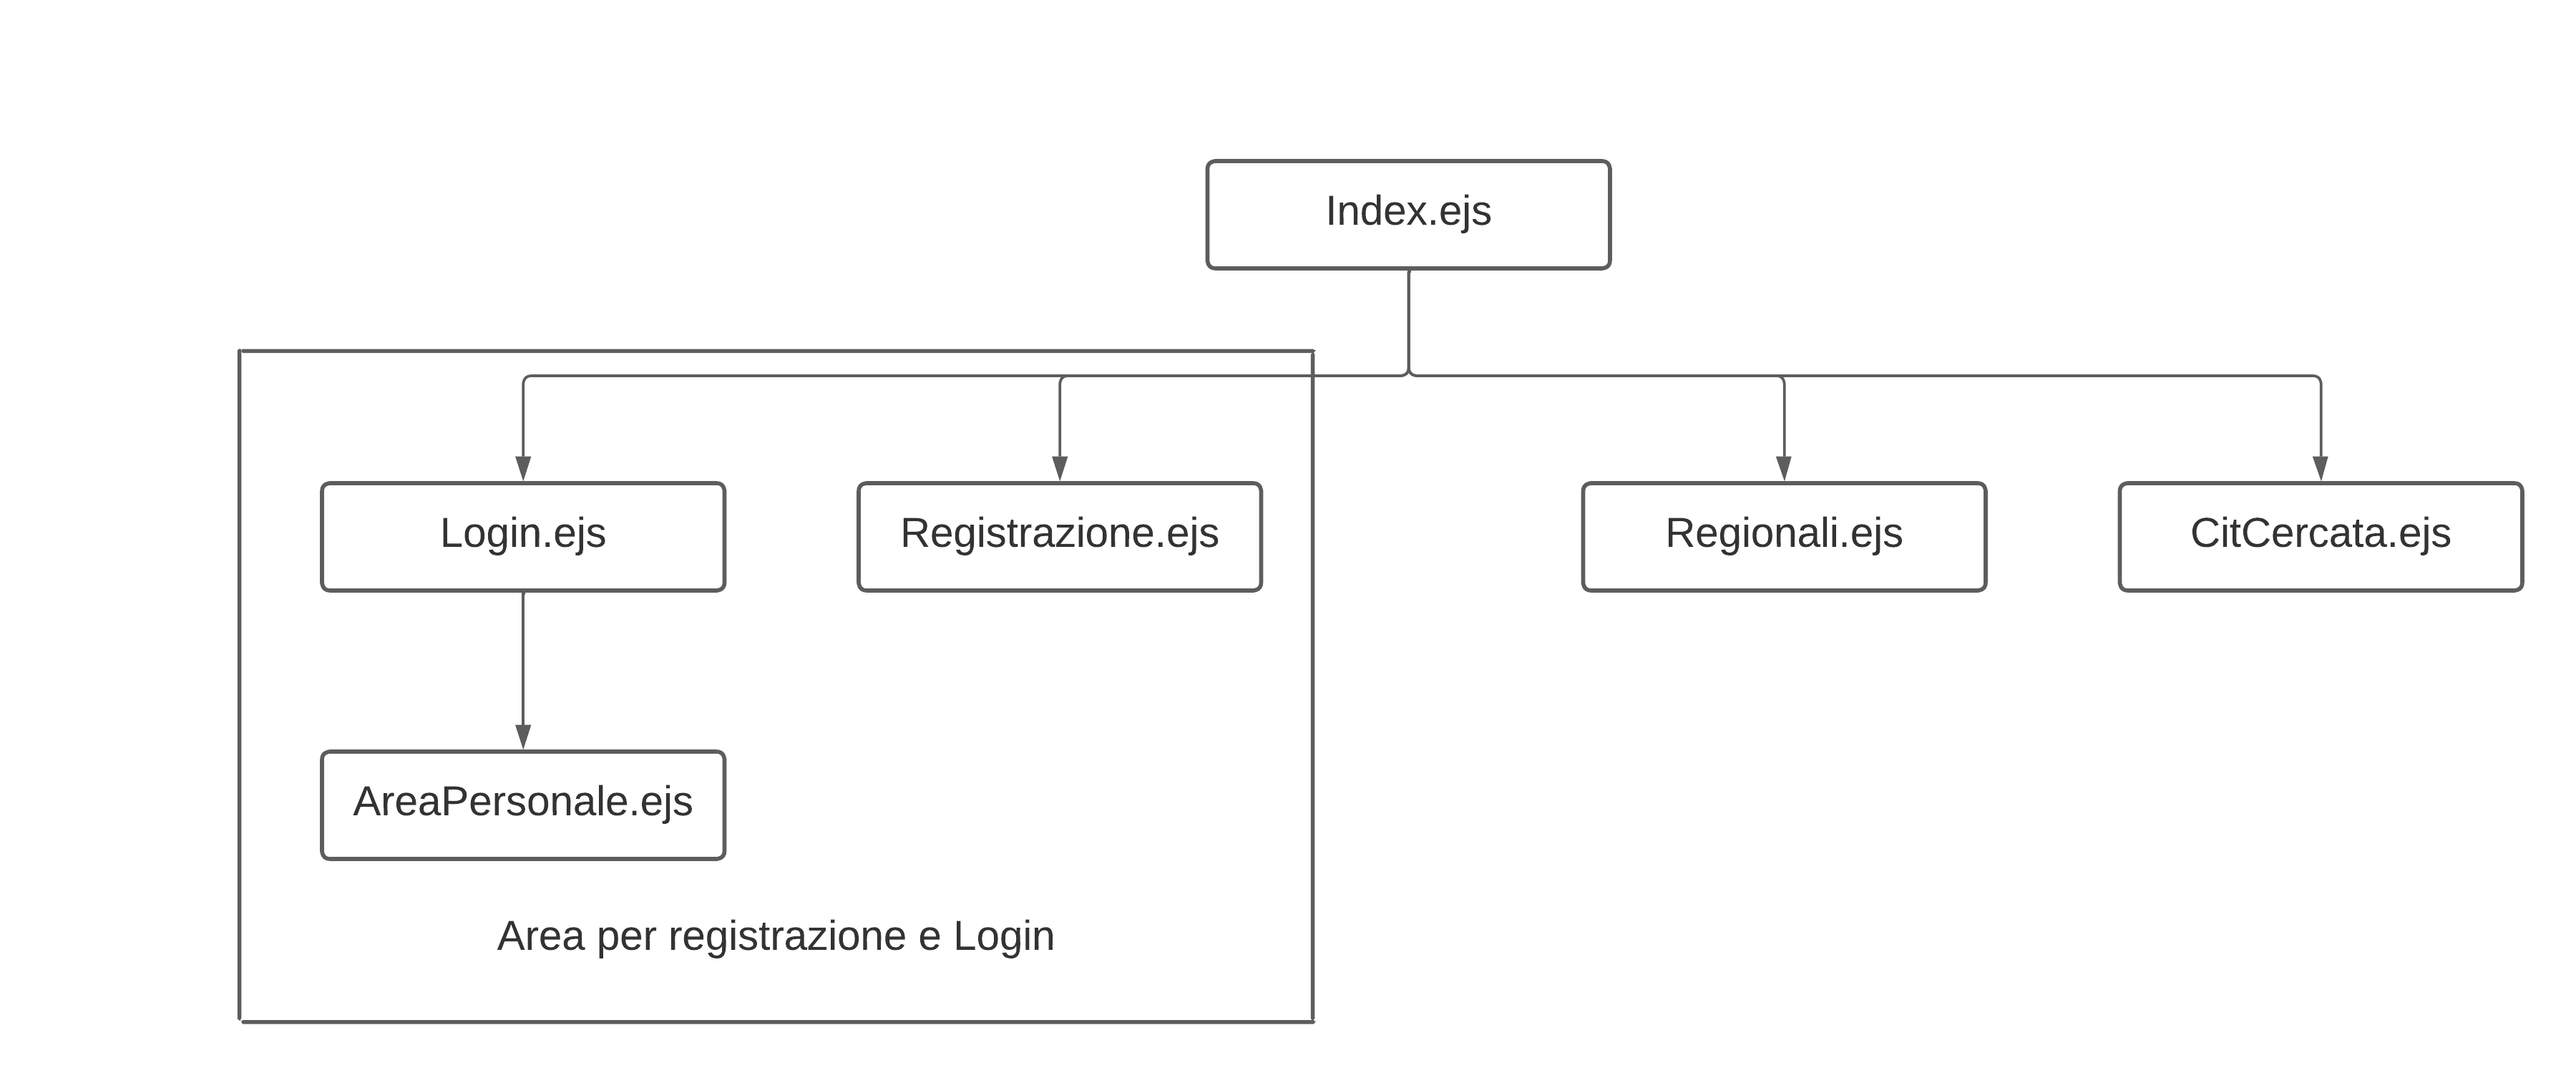
\includegraphics{img/architettura.png}}
    \caption{Architettura gerarchica delle pagine}
\end{figure}

Il punto di accesso al sito è pensato per essere costituito dall'index. Attraverso di essa sarà infatti 
possibile accedere tramite uno o più passaggi a tutte le pagine del sito (la navigazione da una pagina all'altra rimane comunque 
sempre disponibile attraverso la navbar, a prescindere da dove ci si trovi nel sito).

\vspace{5mm}

Per accedere alla pagina \emph{AreaPersonale.ejs} e a qualunque funzione che richieda di essere loggati, 
sarà necessario aver effettuato realmente il login: in caso contrario, la richiesta verrà rifiutata dal 
server.

\section{Routing lato server}

Le route previse dal server sono:
\begin{itemize}
    \item \emph{/} (GET): index. Nel caso in cui si sia autenticati (attraverso un cookie), verrà modificata la 
    navbar in modo da mostrare un menù a tendina per entrare nell'area personale al posto di quello per l'autenticazione; 
    questo viene realizzato modificando il JSON inviato a EJS per renderizzare la pagina;
    \item \emph{/login} (GET): pagina di login. Nel caso il login vada a buon fine, si verrà reindirizzati all'index; altrimenti, 
    si verrà reindirizzati a \emph{/login?auth=fail}, query che permette di mostrare un messaggio di errore;
    \item \emph{/verificaCredenziali} (GET): indirizzo raggiunto dal form nella pagina di login per verificare le credenziali 
    inserite;
    \item \emph{/registrazione} (GET): pagina per la registrazione. Sia che la registrazione vada a buon fine sia che dia errore, 
    verrà mostrato un messaggio in relazione al risultato ottenuto dal server. Per effettuare il login bisognerà usare la pagina 
    apposita;
    \item \emph{/creaUtente} (POST): indirizzo raggiunto per creare un nuovo utente;
    \item \emph{/areaPersonale} (GET): pagina relativa all'area personale;
    \item \emph{/aggiornaDati} (POST): indirizzo raggiunto per modificare i dati relativi all'utente registrato;
    \item \emph{/aggiornaCit} (POST): indirizzo usato per aggiungere una città dai preferiti;
    \item \emph{/rimuoviCit} (PUT): indirizzo usato per rimuovere una città dai preferiti;
    \item \emph{/logout} (GET): indirizzo usato per eliminare il cookie usato per autenticare l'utente;
    \item \emph{/citCercata} (GET): indirizzo usato per verificare se la città cercata esista o meno;
    \item \emph{/meteoCitCercata} (GET): pagina che mostra il meteo in tempo reale della città cercata;
    \item \emph{/previsioniRegionali} (GET): pagina per mostrare le previsioni di tutte le regioni;
    \item \emph{/previsioniRegionali/regione} (GET): indirizzo raggiunto per ottenere le province di una data regione.
\end{itemize}

\subsection{Descrizione delle risorse}

\subsubsection{Database}

Il motore utilizzato per realizzare il database è MongoDB.\\
Il database si compone di un'unica collezione (chiamata \emph{users}), utilizzata per salvare i dati relativi agli utenti registrati. 
Ogni documento, come anticipato nell'introduzione, avrà la seguente struttura:
\begin{itemize}
    \item \emph{\_id}: id univoco assegnato dal database in automatico;
    \item \emph{user}: username;
    \item \emph{email}: email dell'utente;
    \item \emph{pw}: password dell'utente sotto forma di digest SHA256;
    \item \emph{pref}: array contenente le città messe tra i preferiti dall'utente. può essere vuoto.
\end{itemize}

\subsubsection{Autenticazione}

L'autenticazione sarà considerata corretta se il digest SHA256 della password e l'email inseriti dall'utente corrisponderanno 
a quelli di un documento presente nel database (si ricorda che username e email sono \textbf{univoci}).

\vspace{5mm}

Nel caso l'autenticazione vada a buon fine, verrà resituito un \emph{cookie} valido per 30 minuti e contente lo username dell'utente. 
Se l'utente dovesse cambiare il suo username all'interno dell'area personale, il contenuto del cookie verà aggiornato. 
\chapter{Codice}

\section{HTML 5}

Il codice di tutte le pagine dell'applicazione è strutturato in modo da avere: 
\begin{itemize}
    \item lo stesso contenuto nel tag head (importato con un partial file);
    \item una navbar contenente:
    \begin{enumerate}
        \item il nome del sito (Meteo);
        \item un link alla Home in modo da poterci sempre tornare in qualunque momento;
        \item un link alla pagina per il meteo in tempo reale delle province di ciascuna regione;
        \item un menù a tendina per autenticarsi/registrarsi oppure per accedere all'area personale/effettuare 
        il logout nel caso in cui si sia già autenticati;
        \item bottone per fare il toggle tra light e dark mode;
        \item barra di ricerca per ottenere il meteo in tempo reale di una città.
    \end{enumerate}
    I punti 3 e 4 non saranno presenti nella navbar delle pagine dedicate a login e registrazione. 
\end{itemize}

\vspace{5mm}

Ogin pagina avrà poi un contenuto personalizzato in base al suo scopo.

\section{CSS3}

Nel progetto non sono stati integrati file \emph{.css} personalizzati in quanto tali funzioni sono state assolte tramite le classi 
di bootstrap.

\section{API}

Nel progetto sono state integrate 3 API:
\begin{itemize}
    \item \emph{openWeather}: API usata per ottenere le condizioni meteo in tempo reale;
    \item \emph{pexels}: API in grado di fornire immagini a partire da una query contenente un filtro che descriva il soggetto mostrato;
    \item \emph{comuni ITA}: API in grado di fornire l'elenco dei comuni presenti in italia, nonché delle regioni e delle province di ogni regione.
\end{itemize}

\section{Node.js}

Il server Node.js, implementato secondo paradigma \emph{RESTful}, mette in pratica tutte le funzionalità descritte nei capitoli precedenti. Viene implementato 
grazie all'uso del framework \emph{Express} e di \emph{MongoDB} per memorizzare i dati degli utenti registrati.\\
La comunicazione avviene tramite l'uso di HTTP e le chiamate asincrone; le chiamate effettuate dal server al database sono anch'esse tutte asincrone.

\vspace{5mm}

Si può utilizzare un file presente in \emph{assets/mongoDB} per configurare il database in automatico.

\vspace{5mm}

Per consultare il file server.js contenente il server in toto e il relatvo codice, 
riferirsi alla repository github \url{https://github.com/MatteoCelardo/progettoPWM} seguendo il percorso \emph{assets/node}.


\section{librerie esterne e JavaScript}

Per consultare tutti i file JavaScript e il relatvo codice, riferirsi alla repository github \url{https://github.com/MatteoCelardo/progettoPWM} 
nel percorso \emph{assets/js}.

L'unica libreria esterna integrata è utilizzata per il calcolo dello SHA256 di una stringa è reperibile al link \url{https://cdnjs.cloudflare.com/ajax/libs/crypto-js/3.1.2/rollups/sha256.js}.
\chapter{Possibili sviluppi e conclusioni}

Come detto in precedenza, l'applicazione si occupa di fornire le condizioni meteo in tempo reale relative ad una o più città italiane.

\vspace{5mm}

Alcuni possibili spunti di sviluppo per accrescere l'efficienza, la sicurezza e l'estetica dell'applicazione potrebbero essere:
\begin{itemize}
    \item introduzione di librerie più efficienti rispetto a quelle attualmente integrate;
    \item efficentamento del codice JavaScript attualmente integrato attraverso un maggiore studio delle funzioni offerte ed eventuale 
    introduzione di apposite librerie per svolgere tali scopi;
    \item introduzione di web worker per effettuare le richieste asincrone al server tramite fetch, caricare le immagini e effettuare 
    il calcolo dello SHA256 delle password inserite dall'utente;
    \item introduzione di un sistema di comunicazione con chiavi SSL per l'utilizzo del protocollo HTTPS;
    \item introduzione di una navbar apposita per i dispositivi mobili.
\end{itemize}

\vspace{5mm}

Alcuni spunti di sviluppo per accrescere il valore commerciale dell'applicazione sono riassumibili in:
\begin{itemize}
    \item introduzione di pubblicità all'interno del sito;
    \item introduzione di un'API per fornire ad altri sistemi il meteo in tempo reale.
\end{itemize}
\chapter{Bibliografia}

\begin{itemize}
    \item API pexels: \url{https://www.pexels.com};
    \item API openWeather: \url{https://www.pexels.com};
    \item API comuni ITA: \url{https://comuni-ita.herokuapp.com};
    \item libreria usata per generare digest SHA256: \url{https://cdnjs.cloudflare.com/ajax/libs/crypto-js/3.1.2/rollups/sha256.js};
    \item repository github con l'intero progetto e la documentazione con LaTex sorgente: \url{https://github.com/MatteoCelardo/progettoPWM};
    \item bootstrap: \url{https://getbootstrap.com}
\end{itemize}

\end{document}